\documentclass[11pt]{article}
\usepackage[utf8]{inputenc}
\usepackage{amsmath,amssymb,hyperref,array,xcolor,multicol,verbatim,mathpazo}
\usepackage[normalem]{ulem}
\usepackage[pdftex]{graphicx}
\usepackage{fullpage}
\usepackage{import}
\usepackage{adjustbox}
\usepackage{booktabs}
\usepackage[font=footnotesize,labelfont=bf]{caption}
\captionsetup{justification=raggedright,singlelinecheck=false}


\usepackage[backend=biber,style=authoryear,
sorting=ynt,citestyle=authoryear]{biblatex}
\addbibresource{papercitations.bib}
\usepackage{setspace}
\onehalfspacing
\addtolength{\skip\footins}{2pc plus 5pt}

\title{Labor Markets and Technological Change: Evidence from Electronic Health Records}
\author{Hanna Glenn}
%\date{\today}

\DeclareLabeldate[online]{%
  \field{date}
  \field{year}
  \field{eventdate}
  \field{origdate}
  \field{urldate}
}

\begin{document}

\maketitle



\vspace{1.5cm}

The relationship between technological innovation and labor markets is a longstanding topic of interest in economics and in policy making. Their interaction is relevant in several aspects: technology causing displacement, whether low-skilled vs. high-skilled workers are differentially impacted, or the productivity gains that can be realized due to technology. In many capacities, across differing countries and industries, people tend to care about how technology affects current and future labor markets. This paper seeks to better understand this relationship under a major technology change in the U.S. healthcare system, the implementation of electronic health care record systems in hospitals. 

Electronic Health Records (EHRs) have become increasingly relevant in the U.S. since 2008, in part after former President Obama stated in 2009, “To improve the quality of our health care while lowering its cost, we will make the immediate investments necessary to ensure that, within five years, all of America’s medical records are computerized.” (\cite{presquote}). The movement towards digitization in health care was expected to have immediate and substantial impacts on cost and quality of care. For example, a 2005 study estimated hundreds of billions of dollars saved if health information technology were to be fully implemented (\cite{hillestad2005}). Improvement in quality of care was expected as a result of physicians having more time to spend with patients, better communication across different physicians on the same care plan, and decision-making assistance to avoid harmful mistakes. Such expectations about cost and quality led the government to incentivize the use of EHRs in hospitals with the the Health Information Technology for Economic and Clinical Health (HITECH) Act in 2008 (\cite{hitech}). This legislation subsidized hospitals which used EHRs “meaningfully”\footnote{According to Quatris Healthco, meaningful use standards proceeded in three stages over time. In Stage 1 (2010), MU focused on data capturing and sharing. In Stage 2, which began in late 2012, MU extended to using EHRs for patient incorporation and using the technology as a helper in care. Stage 3 went from 2014-2016 and focused on making data accessible across hospitals (\cite{meanuse})}. The movement towards EHR use is evidenced in hospitals from 2008 onward; the percentage of hospitals with the capability of using a basic EHR system went from 9 percent in 2008 to 84 percent in 2015 (\cite{stats}).

Specifically, an EHR is digital version of a patient’s medical records. These include detailed accounts and notes of medical history and can become advanced enough to provide the physician suggestions for care. Physicians are the primary users of this technology and have a significant role in determining whether potential benefits of EHRs are realized. However, the day-to-day life of physicians changed drastically with the rapid implementation of EHRs. What was expected to be a helpful tool turned out to be burdensome and frustrating for the persons using it. In individual interviews, multiple physicians reported that when using EHRs they are less satisfied with their job and have higher burnout and higher stress levels. Senior physicians in particular were found to “loathe the cumbersome, time-consuming data entry that comes with using EHRs.” (\cite{CollierBurnout}). A physician with the choice to retire or move to a smaller private practice may choose to do so when the cost of using an EHR in a hospital becomes too high. This paper seeks to understand whether the implementation of EHRs in hospitals led to changes in physician labor market outcomes: where to work, productivity levels, and retirement.

Using CMS Shared Patient Data from 2009-2015, I construct a panel of physician-hospital pairs that captures a specific working relationship between the pair, most likely the physician working in the hospital. I link the hospitals to AHA survey data for information on EHR use and then aggregate the data to the physician level. The key independent variable for my main analysis is an individuals physicians' exposure to electronic health records. There are three outcomes of interest in this paper. First, I consider the decision for a physician to retire. \textcolor{red}{This is measured using blank}. Second, I consider whether those physicians who stay in the labor force choose to substitute work towards office-based practices. \textcolor{red}{This information comes from blank.} Finally, for physicians who continue working in hospitals, I analyze the productivity impacts of EHRs. The measure of productivity used is the number of Medicaid patients that bill the both the physician and a hospital in the same day, which comes from the CMS Shared Patient Data. 

The estimation is an event-study approach, where treatment is whether a physician is exposed to an EHR. I assume the decision of a hospital to implement an EHR is exogenous to the physician, but explore this assumption in more detail in Section \textcolor{red}{blank}. \textcolor{red}{To extend the analysis I also utilize difference in difference with continuous treatment, using fraction of hospitals using an EHR as the treatment variable.}  

\textcolor{red}{Paragraph about findings}

This paper contributes to the general understanding of two main questions: the broad effects of technology on labor markets, and the more specific effects of EHR implementation in various healthcare dimensions.

How technology affects labor market outcomes depends drastically on the industry and setting being considered. Health is a major component of expense in the United States, accounting for approximately 17 percent of GDP. Within the health sector, health information technology has been a major change implemented widely. There is a continual discussion amongst policymakers and researchers about how to lower healthcare spending without sacrificing quality of care. Thus, the potential cost savings of EHRs are extremely important to understand given their potential to also improve patient satisfaction, since there is a continual interest in achieving these two things simultaneously. Further, there is the question in both economics and medical literature of whether there exists a physician shortage and, similarly, access to care issues in the U.S. (\cite{cooper2002economic}). A relevent factor of this discussion is whether electronic health records are driving physicians out of the market or decreasing the amount of patients that can be seen by one physician, both of which have the potential to worsen these issues.

The effects of EHR implementation on costs and quality of healthcare prior to 2010 have been studied extensively. Despite many case studies and hospital-level analysis that indicate large improvements in health outcomes such as mortality (\cite{Buntin2011TheResults}), more recent economic research has showed that the technology has only improved health outcomes for patients with severe conditions, but have not led to improvements for the median patient (\cite{Agha2014TheCare}; \cite{McCullough2016HealthCoordination}; \cite{Meyerhoefer}). Further, there have been no significant cost decreases due to EHRs in the short or long run. If any cost reductions are realized at all, they are at least 6 years after implementation (\cite{dranove2014trillion}). However, the incentive programs put in place could impact the cost effects of EHRs, and 6 years may not be a long enough time frame to see the full picture of cost effects. While this paper does not specifically investigate hospital costs, it does speak to potential drivers of cost effects. Finally, there have been preliminary case studies and interviews seeking to understand physicians' outlook on EHRs. These differ depending on the setting studied, where there is evidence of older physicians having more frustration regarding the technology than younger physicians. \textcolor{red}{I need a citation here and probably to expand more on the idea of physician opinions.}

This paper's contribution to the space is threefold: (1) this is the first study to my knowledge that empirically analyzes the relationship between physician labor markets and EHRs, (2) since there seems to be a disconnect between the potentials of EHR technologies and the realized effects, this paper will speak to a potential mechanism that is causing this puzzle, and (3) this study covers the time period of the major EHR boom in healthcare, whereas most studies mentioned above utilize data before 2010, capturing more so the effect of computerization.


\section{Background}

\textcolor{red}{Need to figure out what goes in this section. History of EHRs? Specifics of the subsidies and meaningful use?}

\section{Data}

Using various linked datasets, I construct a physician-level panel spanning from 2009-2015 which measures physicians' exposure to EHRs over time and other relevant characteristics. The different data sets used to construct this panel are described below.

The main data I utilize is the CMS Shared Patients Data. For a pair of National Provider Identifiers (NPIs), it records the number of patients who bill both of the entities under Medicaid in the same day. For example, if a Medicaid patient is referred to a specialist by a primary care physician, then those two physicians have a shared patient in common. I limit the entities to only include the number of shared patients for physician-hospital pairs. I care specifically about physicians who have a close working relationship with hospitals, preferably those who do rounds within at least one hospital. To achieve this, I limit the qualifications for a sufficient physician-hospital pair. First, I only consider doctors who have a primary care role, excluding any specialists. The reason for this is that a primary care physician who does rounds in a hospital is likely to be primarily employed by that hospital (not brought in from a practice). Another reason for this is that primary care doctors interact directly with EHRs during checkups, unlike a surgeon. Second, I limit pairs to those which have a substantial number of patients billed together in the same day. This is to avoid including the potential physician who works in an office but happens to send a small number of patients to a nearby hospital. I consider a substantial number of patients to be at least 30 patients bill both the physician and the hospital in the same day in at least one year, \textcolor{red}{where the exact number chosen is explored in the appendix}. The physicians remaining in the data are likely doing a number of rounds physically inside hospitals, since it is unlikely that many patients will see a primary care doctor in a private office and then immediately go to a hospital in the same day. 

Using hospital NPI, I link the physician-hospital pairs to the American Hospital Association survey, which contains information on hospital-level EHR use and other characteristics. I then aggregate to the physician level, where physician EHR use is measured as the percentage of their hospitals which use an EHR in a given year. Additional physician-level characteristics, such as years of experience, come from Physician Compare. 

Overall summary statistics of the variables are shown in \hyperref[fig:summarystatistics]{Table 1}. Average hospital operating days is a physician-level variable that averages the number of operating days for that physicians hospital network. While there are some low outliers with a low value, on average physicians are working in hospitals open year round. Similarly, the average size of the hospital worked with averages the number of beds of each hospital in a physician's network. While these two average variables can technically vary by year, they tend to stay constant across the data, which is why they are included in the static category. Approximately 30\% of the sample of physicians are female and the average physician graduated medical school in 1993. Note that there are no physicians in the data who graduated after 2009, since they would be entering the labor force during the span of the data. On average, a physician works with between 1 and 2 hospitals as well as hospital systems. While the number of hospitals that a physician cares for patients in varies by year, the number of hospitals in their network is constant. The physician level variables that vary over time deal are the treatment variables regarding EHR exposure and the number of Medicaid patients seen. For all physician-years, physicians were exposed to an EHR in 56\% of the hospitals they work in and 70\% of the sample is exposed to any EHR. Once a physician becomes exposed to an EHR, they cannot go back to being unexposed. Finally, physicians are seeing an average of 620 Medicaid patients in hospitals per year. \textcolor{red}{In Appendix A1, I include summary statistics by subsample of physician age and year.} 


\begin{table}[ht]
    \import{Table Code}{overall stats.tex}
    \label{fig:summarystatistics}
    \vspace{1mm}
    \caption*{\footnotesize Obs: 1,044,001}
\end{table}



For a clear look at the variation in treatment variables over time, \hyperref[fig:figure1]{Figure 1} shows the average of these variables over time. In 2009, 42\% of the sample of physicians were exposed to an EHR. That is, over half of the sample had no affiliation with EHRs at the beginning of the sample period. By 2015, 92\% of physicians had exposure to an EHR in at least one hospital in their network. Similarly, the fraction of hospitals in a physician's network which were using an EHR was 30\% in 2009 and grew to 82\% in 2015. These statistics are consistent with the surge in incentives to implement EHRs in hospitals. 

\begin{figure}
    \caption{Treatment Variables Over Time}
    \vspace{-2mm}
    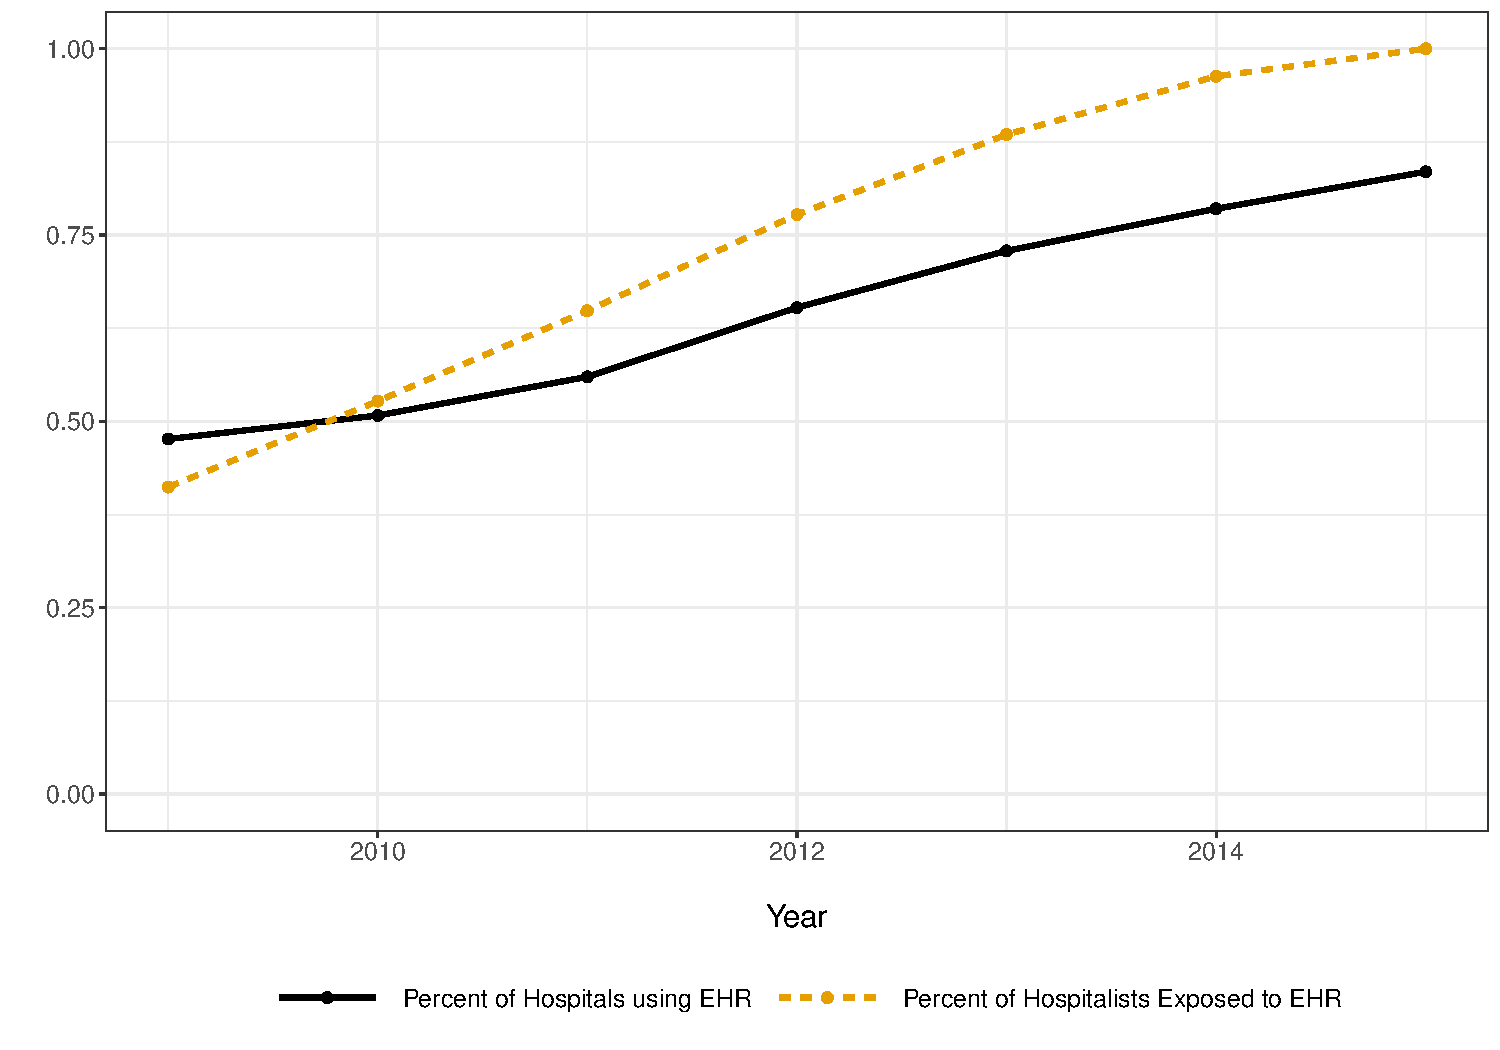
\includegraphics[scale=.5]{Objects/sum_stats_year.pdf}
    \label{fig:figure1}
\end{figure}



\section{Retirement}

\section{Work Setting}

\section{Physician Productivity}

An important aspect in the implementation of EHRs is whether or not they increase productivity in users. Productivity, in this case, has two key determinants: the choice of physicians to learn and utilize the technology, and the realized quality/innovation of electronic health records themselves. Regarding the first determinant, I will assume that when a physician continues to work in an electronic record utilizing-hospital, they utilize the electronic health record system fully. That is, there are no physicians who stay actively working in a hospital but choose not to partake in the electronic health record used by the hospital. To understand the second determinant, the value added of electronic health records themselves, the sample of physicians is limited to those who have patients in hospitals even after EHR exposure. 

It is reasonable to believe that physicians are fully utilizing the EHRs in the hospital they work in, since by 2015 electronic health records were widely implemented and considered unavoidable. An objection to this assumption may be that older physicians stay in a hospital, but the hospital hires a data assistant to do technology work for the physician. In this cae, the productivity gain could be from having the data assistant instead of EHR use. I investigate this below.

\subsection{Data Assistants}

\textcolor{red}{get data from AHA on data assistance. It may be that I just need to show a graph here of the number of data assistant jobs at hospitals. Need to see from there. }

\subsection{Event Study and Results}

The analysis in this section focuses on the effects of hospital EHR implementation on physician productivity within hospitals, measured by the total number of Medicaid patients billed in hospitals in a given year. The estimating equation is given as follows: 

\begin{equation*}
    y_{it}=\alpha_i+\delta_t+q_{it}'\lambda+\sum_{k=-5}^5 \beta_kz_{i,t-k} + \varepsilon_{it},
\end{equation*}

where $y_{it}$ is the number of patients, $\alpha_i$ and $\delta_i$ are physician and time fixed effects, $q_{it}$ are hospital characteristics such as number of beds and days open during the year, $z_{i,t-k}$ is an indicator for whether the physician was exposed to an EHR in any hospital in time $t-k$, and $\epsilon_{it}$ is a random error term. 

The identifying assumption is that physicians are exposed endogenously to electronic health records. That is, hospital management decides and implements EHRs, and this decision is not correlated with physician productivity or labor market decisions. This is not unreasonable for large hospitals with ample resources and many physicians. However, a small hospital may give experienced physicians some level of voice in the decision to implement new technologies. Results under this assumption are shown below, and  \textcolor{red}{the strength of this assumption is considered in the next section. } 

An event study plot containing estimates and confidence intervals of  $\{\beta_k\}_{k=-5}^5$  is given in in Figure \textcolor{red}{number}. The left hand side is the full sample of physicians at any experience level. As is standard in event studies, the identification of the coefficients depends on the assumption that there are no pre-trends. The p-value of a Wald test for pre-trends in both event studies indicate no observable pre-trends in the data.

For physicians at any experience level, EHR exposure yields no immediate affect on physician productivity, but leads to a clear increase in the number of patients seen beginning 2 years after exposure. After 5 years of exposure, physicians are seeing, on average, 93.67 more Medicaid patients per year. Relative to the mean in the year before exposure, 796.95, this is an 11.75\% increase in the number of patients seen. When the sample of physicians is limited to senior physicians (at least 35 years of experience), this effect disappears. In fact, the results show a slight decrease of \textcolor{red}{put the exact number here} in the number of patients seen in the year after exposure, and no effect following that year. This graph limits event time from -4 to 4 due to restricted sample size in year 2010 and 2014. 


\begin{figure}[ht]
\caption{}
        \begin{minipage}[b]{0.47\linewidth}
            \centering
            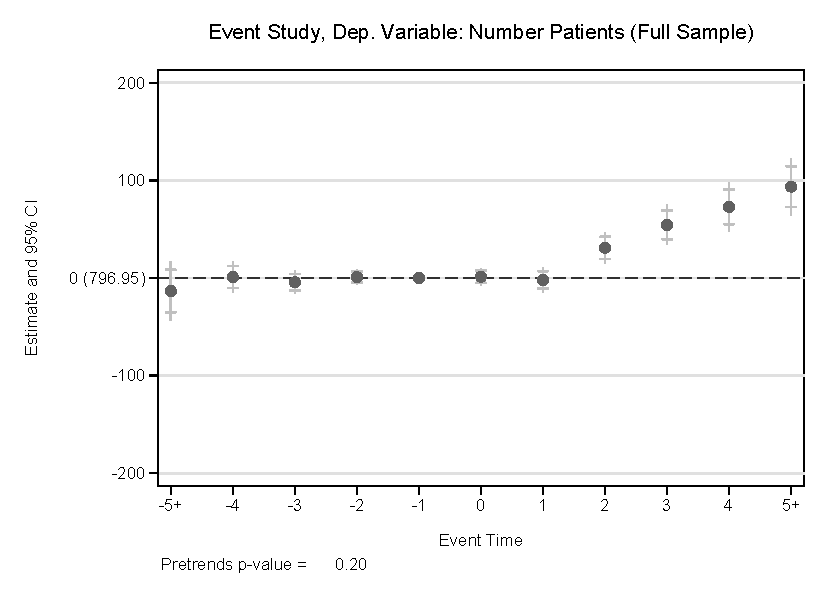
\includegraphics[width=\textwidth]{Objects/prod_eventstudy_fullsample.pdf}
        \end{minipage}
        \hspace{0.2cm}
        \begin{minipage}[b]{0.47\linewidth}
            \centering
            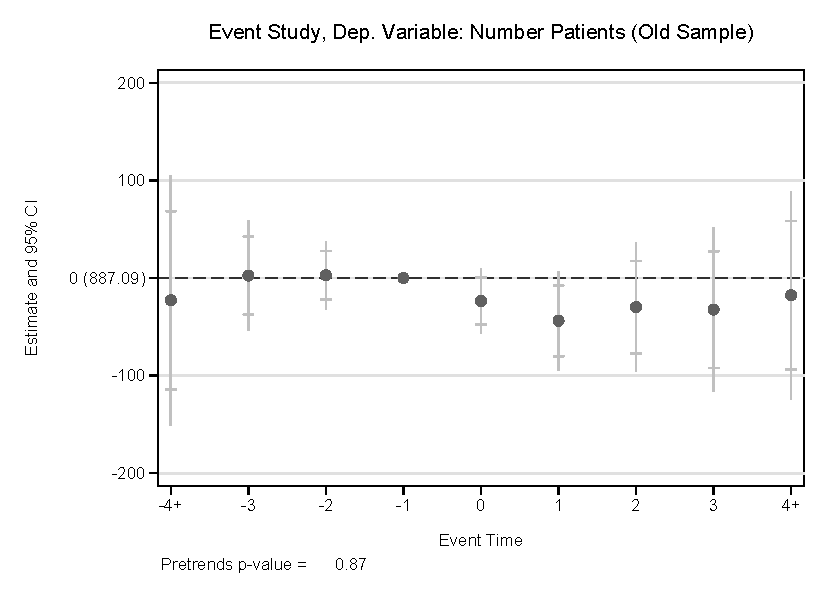
\includegraphics[width=\textwidth]{Objects/prod_eventstudy_oldsample.pdf}
        \end{minipage}
\end{figure}

\subsection{Relaxing Exogeneity of Implementation}


\textcolor{red}{I need to put somewhere that i dropped 2015 for this analysis since it cut off at a different point than the other years}


\end{document}